\documentclass{beamer}
\input{myBeamerPackage.tex}

\usepackage[style=verbose,backend=bibtex]{biblatex}
\addbibresource{flandersMakeApplicatie.bib}

\title[Flanders make presentation]%\hspace{1cm} \insertframenumber/\inserttotalframenumber]
{Flanders make job interview:\\IIoT enabled manufacturing of multi material machine canopies}

\author[Tijl]
{Tijl Jappens \\
	\scriptsize KU Leuven}


\institute[]{
	instituut voor theoretische fysica KU Leuven
}


\date{\today}

\setbeamertemplate{itemize items}{\color{black}$\triangleright$}
\setbeamertemplate{enumerate items}{\color{black}\insertenumlabel.}

\usepackage[T1]{fontenc}
\DeclareRobustCommand{\augiefamily}{%
	\fontfamily{augie}\fontseries{m}\fontshape{n}\selectfont}
\DeclareTextFontCommand{\textaugie}{\augiefamily}

\begin{document}
	
	%%%%%%%%%% Removes the frame number from the title page %%%%%%%%%%
	\bgroup
	\makeatletter
	\setbeamertemplate{footline}
	{
		\leavevmode%
		\hbox{%
			\begin{beamercolorbox}[wd=.333333\paperwidth,ht=2.25ex,dp=1ex,center]{author in head/foot}%
				%   \usebeamerfont{author in head/foot}\insertshortauthor\expandafter\beamer@ifempty\expandafter{\beamer@shortinstitute}{}{~~(\insertshortinstitute)}
			\end{beamercolorbox}%
			\begin{beamercolorbox}[wd=.333333\paperwidth,ht=2.25ex,dp=1ex,center]{title in head/foot}%
				%    \usebeamerfont{title in head/foot}\insertshorttitle
			\end{beamercolorbox}%
			\begin{beamercolorbox}[wd=.333333\paperwidth,ht=2.25ex,dp=1ex,right]{date in head/foot}%
				%    \usebeamerfont{date in head/foot}\insertshortdate{}\hspace*{2em}
				%    \insertframenumber{} / \inserttotalframenumber\hspace*{2ex} 
		\end{beamercolorbox}}%
		\vskip0pt%
	}
	\makeatother
	\begin{frame}
		\titlepage
	\end{frame}
	\egroup
	
	\begin{frame}{Machine canopies}
		\centering
		\includegraphics[width=0.8\textwidth]{Figures/examples of canopies.pdf}
	\end{frame}

	\begin{frame}{Understanding the current situation}
		\begin{enumerate}
			\item Adapting production line?
			\item Modifiable parameters?
			\pause
			\item Measuring quality?
			\item Regulations that have to be satisfied?
			\pause
			\item Process if machine has downtime?
			\pause
			\item Manuals, guidelines, procedures or historical records?
		\end{enumerate}
	\end{frame}

	\begin{frame}{The manufacturer's goals}
		\begin{enumerate}
			\item Making system future proof.
			\item Follow production orders.
			\item Trace production (log data of steps).
			\item Monitor performance and display in some dashboard.
			\item Use data to optimize production.			
		\end{enumerate}
	\end{frame}

	\begin{frame}{Production process}
		\begin{enumerate}
			\item Thermoforming.
			\item Deburring.
			\item Surface preparation.
			\item Mixing adhesive.
			\item Application of the adhesive.
			\item Curing joint.
			\item Assembly of optional features.
		\end{enumerate}
	\end{frame}
	
	\begin{frame}{Literature study:\\Deep learning for the quality control of thermoforming food packages\footcite{Banus2021}}
		\centering
		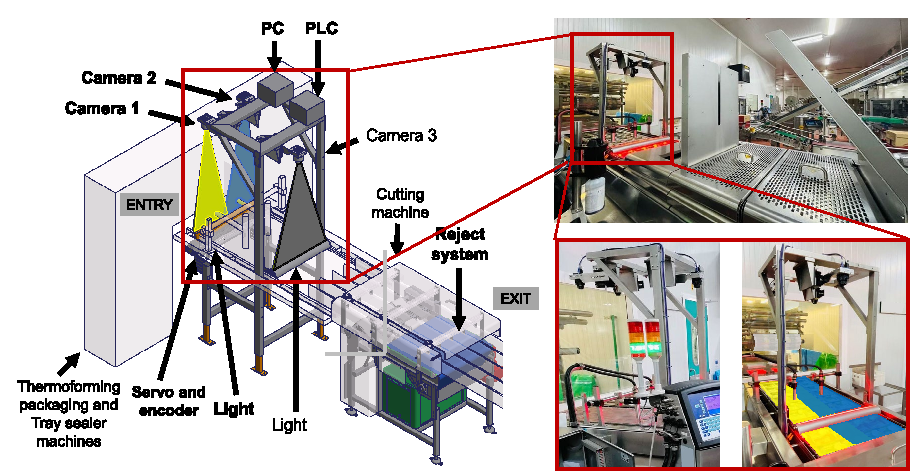
\includegraphics[width=0.8\textwidth]{Figures/QualityControlInThermoformingSetup.pdf}
	\end{frame}

	\begin{frame}{Literature study:\\Deep learning for the quality control of thermoforming food packages}
		\begin{itemize}
			\item Used transfer learning.
			\item Started from various Convolutional Neural Networks.
			\item Detects and categorizes defects.
		\end{itemize}
		\centering
		\includegraphics[width=0.8\textwidth]{Figures/DefectsOfPlastic.pdf}
	\end{frame}
	
	\begin{frame}{Literature study:\\Deep learning for the quality control of thermoforming food packages}
		Is this useful for the problem at hand?
		\pause
		\begin{itemize}
			\item There were large amounts of widely available data. De we get access to such things?
			\pause
			\item If the parameters are changed do we have to retrain the system?
			\pause
			\item Does this method work for every type of plastic?
			\pause
			\item Aren't there just far simpler image recognition techniques that do this job? Probably, I don't know.
		\end{itemize}
	\end{frame}

	\begin{frame}{Literature study:\\Derivation of processing parameters of polypropylene foam thermoforming by an artificial neural network\footcite{https://doi.org/10.1002/pen.20287}}
		\centering
		\includegraphics[width=0.8\textwidth]{Figures/FoamCupThemoformingProcess.pdf}
	\end{frame}

	\begin{frame}{Literature study:\\Deep learning for the quality control of thermoforming food packages}
		\begin{columns}
			\begin{column}{0.5\textwidth}
				\begin{center}
					\includegraphics[width=\textwidth]{Figures/CupProcessNoExplenation.pdf}
				\end{center}
			\end{column}
			\begin{column}{0.5\textwidth}  %%<--- here
				Parameters of process:
				\begin{enumerate}
					\item Heater temperature.
					\item Plug displacement.
					\item Vacuum time.
					\item Vacuum pressure.
					\item Plug velocity.
					\item Plug material type (heat transfer coefficient).
				\end{enumerate}
			\end{column}
		\end{columns}
	\end{frame}

	\begin{frame}{Literature study:\\Deep learning for the quality control of thermoforming food packages}
		\begin{columns}
			\begin{column}{0.5\textwidth}
				\begin{center}
					\includegraphics[width=0.9\textwidth]{Figures/CupDimensions.pdf}
				\end{center}
			\end{column}
			\begin{column}{0.5\textwidth}  %%<--- here
				Thickness of cup at 6 sites.
			\end{column}
		\end{columns}
	\end{frame}

	\begin{frame}{Literature study:\\Deep learning for the quality control of thermoforming food packages}
		\begin{center}
			\includegraphics[width=0.6\textwidth]{Figures/NeuralNet.pdf}
		\end{center}
		\begin{itemize}
			\item \textbf{Input:} Thicknesses.
			\item \textbf{Output:} Parameters.
			\item \textbf{Training data:} Actual data from cups.
		\end{itemize}
	\end{frame}

	\begin{frame}{Can this be used here?}
		\begin{itemize}
			\pause
			\item Our case seems far more complicated.
			\pause
			\item Other parameters in the optimization process like price, electricity consumption and time.
			\pause
			\item Paper is from 2005. What is the state of the art with these things?
			\pause
			\item I tried to read more modern papers but they contained complicated material sciences.
		\end{itemize}
	\end{frame}
	
	\begin{frame}{}
		content
	\end{frame}
	
	\begin{frame}
		\printbibliography
	\end{frame} 
\end{document}